%%%%%%%%%%%%%%%%%%%%%%%%%%%%%%%%%%%%%%%%%%%%%%%%%%
\section{Model Architectures}
\label{app:sec:architectures}
%%%%%%%%%%%%%%%%%%%%%%%%%%%%%%%%%%%%%%%%%%%%%%%%%%

\begin{figure}[t]
    \centering
    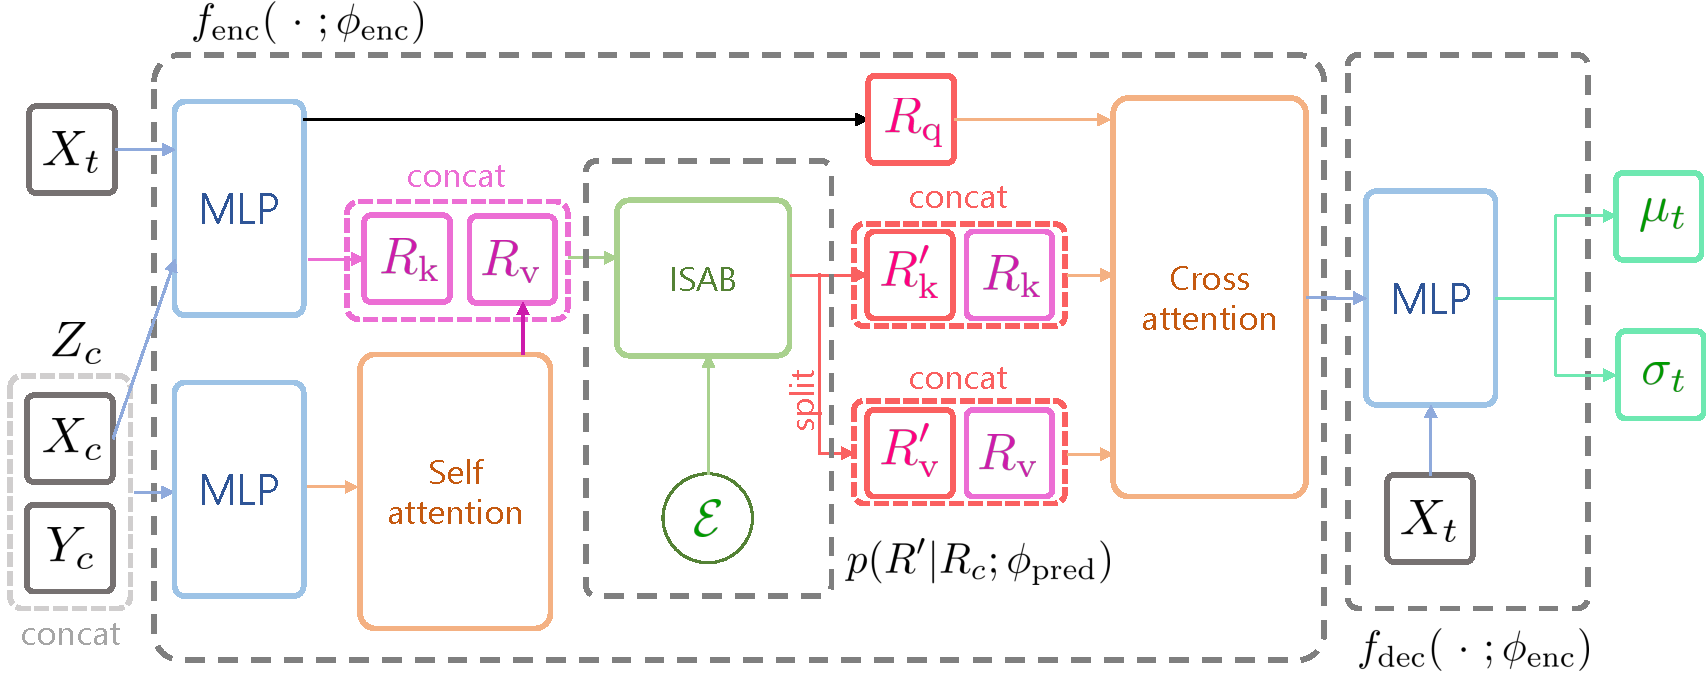
\includegraphics[width = \linewidth]{figure/main_concept_mpanp.pdf}
    \caption{Concept figure of our feature generating model applied to \gls{canp}~\citep{kim2018attentive}. Here we sample $\epsilon$ from a simple distribution (e.g. Gaussian). We generate key feature $R_k'$ and value feature $R_v'$ for cross attention layer which are corresponding to pseudo context data. We use generator as one layer \gls{isab}~\citep{lee2019set} in our experiment.
    %\ed{This figure is awesome!!}}
    }
    \label{figure/main_concept_mpanp}
\end{figure}

In this section, we summarize the model architectures which we used in experiments.
Here, we only present simplified structures for each model.
To see exact computation procedures for \glspl{bnp}, please refer to \citet{lee2020bootstrapping}. \cref{figure/main_concept_mpanp} shows our method applying to \gls{canp} model~\citep{kim2018attentive}.
% To see exact computation procedures for \glspl{bnp} and \glspl{neubnp}, please refer to \citet{lee2020bootstrapping} and \citet{lee2022neural} respectively.

%%%%%%%%%%%%%%%%%%%%%%%%%%%%%%%%%%%%%%%%%%%%%%%%%%
\subsection{Modules}

\paragraph{Linear Layer} $\Lin(d_{\In},d_{\out})$ denotes the linear transformation of the input with dimension $d_{\In}$ into the output with dimension $d_{\out}$.
\paragraph{Multi-Layer Perceptron} $\MLP(n_l, d_{\In}, d_{\hid}, d_{\out})$ denotes a multi-layer perceptron with the structure:
\begin{align*}
    \MLP(n_l, d_{\In}, d_{\hid}, d_{\out}) = \Lin(d_{\hid}, d_{\out})\circ(\ReLU\circ\Lin(d_{\hid},d_{\hid}))^{n_l-2}\circ\ReLU\circ\Lin(d_{\In},d_{\hid}),
\end{align*}
where $\ReLU$ denotes the element-wise Rectified Linear Unit (ReLU) activation function.
\paragraph{Multi-Head Attention} $\MHA(n_{\head}, d_{\out})(Q,K,V)$ denotes a multi-head attention~\citep{vaswani2017attention} with $n_{\head}$ heads which takes input as $(Q,K,V)$ and outputs the feature with dimension $d_{\out}$.
The actual computation of $\MHA(n_{\head}, d_{\out})(Q,K,V)$ can be written as follows:
\begin{align*}
    (Q_i')_{i=1}^{n_\head} &= \spl(\Lin(d_q,d_\out)(Q), n_\head)\\
    (K_i')_{i=1}^{n_\head} &= \spl(\Lin(d_k,d_\out)(K), n_\head)\\
    (V_i')_{i=1}^{n_\head} &= \spl(\Lin(d_v,d_\out)(V), n_\head)\\
    H &= \concat([\softmax(Q_i'K_i'^\top/\sqrt{d_\out})V_i']_{i=1}^{n_\head})\\
    O &= \LN(Q'+H)\\
    \MHA(n_\head,d_\out)(Q,K,V) &= \LN(O+\ReLU(\Lin(d_\out,d_\out)(O)))
\end{align*}
where $(d_q, d_k, d_v)$ denotes the dimension of $Q,K,V$ respectively, $\spl$ and $\concat$ are the splitting and concatenating $A$ in the feature dimension respectively, and $\LN$ denotes the layer normalization~\citep{ba2016layer}.
\paragraph{Self-Attention} $\SA(n_\head, d_\out)$ denotes a self-attention module which is simply computed as $\SA(n_\head, d_\out)(X) = \MHA(n_\head, d_\out)(X,X,X)$.
\paragraph{Multi-head Attention Block} $\MAB(n_\head, d_\out)$ denotes a multi-head attention block module~\citep{lee2019set} which is simply computed as $\MAB(n_\head, d_\out)(X,Y) = \MHA(n_\head, d_\out)(X,Y,Y)$.
\paragraph{Induced Set Attention Block} $\ISAB(n_\head, d_\out)$ denotes a induced set attention block~\citep{lee2019set} which constructed with two stacked $\MAB$ layers.
The actual computation of $\ISAB(n_\head, d_\out)(X,Y)$ can be written as follows:
\begin{align*}
    H &= \MAB(n_\head, d_\out)(Y, X)\\
    \ISAB(n_\head, d_\out)(X,Y) &= \MAB(n_\head, d_\out)(X, H).
\end{align*}

%%%%%%%%%%%%%%%%%%%%%%%%%%%%%%%%%%%%%%%%%%%%%%%%%%
\subsection{\texorpdfstring{\gls{cnp}, \gls{np}, \gls{bnp}, \gls{neubnp} and \gls{mpnp}}{CNP, NP, BNP, NeuBNP, and MPNP}}

\paragraph{Encoder}
The models only with a deterministic encoder (\gls{cnp}, \gls{bnp}, \gls{mpnp}) use the following structure:
\begin{align*}
    r_c &= \frac{1}{|c|} \sum_{i \in c} \MLP(n_l=5, d_{\In}=d_z, d_{\hid}=128, d_{\out}=128)(z_i), \\
    f_\text{enc}(Z_c) &= r_c.
\end{align*}
For the \gls{mpnp}, $f_\enc(Z_c)$ changes into $\concat([r_c,r_c'])$ where $r_c'$ is the feature of the pseudo context data generated from generator in paragraph \textbf{Generator}.
The model also with a latent encoder (\gls{np}) uses:
\begin{align*}
    r_c &= \frac{1}{|c|} \sum_{i \in c} \MLP(n_l=5, d_{\In}=d_z, d_{\hid}=128, d_{\out}=128)(z_i), \\
    (m_c, \log s_c) &= \frac{1}{|c|} \sum_{i \in c} \MLP(n_l=2, d_{\In}=d_z, d_{\hid}=128, d_{\out}=128 \times 2)(z_i), \\
    s_c &= 0.1 + 0.9 \cdot \text{softplus}(\log s_c), \\
    h_c &= \calN(m_c, s^2_c I_h), \\
    f_\text{enc}(Z_c) &= [r_c; h_c],
\end{align*}
where $d_z = d_x + d_y$ denotes the data dimension.
Data dimensions vary through tasks, $d_x=1, d_y=1$ for 1D regression tasks, $d_x=2, d_y=1$ for MNIST image completion task,  $d_x=2, d_y=3$ for SVHN and CelebA image completion tasks, and $d_x=1, d_y=2$ for Lotka Volterra task.

\paragraph{Adaptation Layer}
\gls{bnp} uses additional adaptation layer to combine bootstrapped representation and the base representation. This can be done with a simple linear layer
\[
    \tilde{r}_c = \Lin(d_{\hid}=128, d_{\hid}=d_x+128)(\tilde{r}_c^{(pre)}).
\]

\paragraph{Decoder}
All models use a single MLP as a decoder.
The models except \gls{np} uses the following structure:
\begin{align*}
    (\mu, \log \sigma) &= \MLP(n_l=3, d_{\In}=d_x + 128, d_{\hid}=128, d_{\out}=2)(\concat([x,r_c])) \\
    \sigma &= 0.1 + 0.9 \cdot \text{softplus}(\log \sigma), \\
    f_\text{dec}(x, r_c) &= (\mu, \sigma),
\end{align*}
and \gls{np} uses:
\begin{align*}
    (\mu, \log \sigma) &= \MLP(n_l=3, d_{\In}=d_x + 128 \times 2, d_{\hid}=128, d_{\out}=2)(\concat([x,r_c,h_c])) \\
    \sigma &= 0.1 + 0.9 \cdot \text{softplus}(\log \sigma), \\
    f_\text{dec}(x, r_c, h_c) &= (\mu, \sigma).
\end{align*}


\paragraph{Generator}
\gls{mpnp} use a single $\ISAB$ module as a generator. The $\ISAB$ uses the following structure: 
\begin{align*}
    \epsilon &= \concat([\epsilon_i]_{i=1}^{n_\gen})\\
    r_c' &= \ISAB(n_\head=8, d_\out=128)(\epsilon,r_c)\\
    f_\gen(r_c) &= r_c'
\end{align*}
where $\epsilon_i$s are i.i.d. sampled from Gaussian distribution with dimension 128 and $n_\gen$ denotes a number of pseudo context data.

%%%%%%%%%%%%%%%%%%%%%%%%%%%%%%%%%%%%%%%%%%%%%%%%%%
\subsection{\texorpdfstring{\gls{canp}, \gls{anp}, \gls{banp} and \gls{mpanp}}{CANP, ANP, BANP, NeuBANP, and MPANP}}

\paragraph{Encoder}
The models only with a deterministic encoder (\gls{canp}, \gls{banp}, \gls{neubanp} and \gls{mpanp}) use the following structure:
\begin{align*}
    r_q &= \MLP(n_l=5, d_{\In}=d_x, d_{\hid}=128, d_{\out}=128)(X), \\
    r_k &= \MLP \qquad \qquad \qquad \qquad '' \qquad \qquad \qquad  \qquad \ (X_c), \\
    r_v^{(\text{pre})} &= \MLP(n_l=5, d_{\In}=d_z, d_{\hid}=128, d_{\out}=128)(X_c), \\
    r_v &= \SA(n_\head=8, d_\out=128)(r_v^{(\text{pre})}), \\
    r_c &= \MHA(n_\head=8, d_\out=128)(r_q, r_k, r_v), \\
    f_\text{enc}(Z_c) &= r_c.
\end{align*}
For the \gls{mpanp}, $f_\enc(Z_c)$ changes into 
\begin{align*}
    r_c &= \MHA(n_\head=8, d_\out=128)(r_q, \concat([r_k,r_k']), \concat([r_v,r_v'])),\\
    f_\enc &= r_c,
\end{align*} where $r_k'$ and $r_v'$ are the key and value features of the pseudo context data generated from generator in paragraph \textbf{Generator}.

\gls{anp} constructed as:
\begin{align*}
    r_q &= \MLP(n_l=5, d_{\In}=d_x, d_{\hid}=128, d_{\out}=128)(X), \\
    r_k &= \MLP \qquad \qquad \qquad \qquad '' \qquad \qquad \qquad  \qquad \ (X_c), \\
    r_v' &= \MLP(n_l=5, d_{\In}=d_z, d_{\hid}=128, d_{\out}=128)(X_c), \\
    r_v &= \SA(n_\head=8, d_\out=128)(r_v'), \\
    r_c &= \MHA(n_\head=8, d_\out=128)(r_q, r_k, r_v), \\
    h_i' &= \MLP(n_l=2, d_{\In}=d_z, d_{\hid}=128, d_{\out}=128 \times 2)(z_i), \\
    h_i &= \SA(n_\head=8, d_\out=128)(h_i'), \\
    (m_c, \log s_c) &= \frac{1}{|c|} \sum_{i \in c} h_i, \\
    s_c &= 0.1 + 0.9 \cdot \text{softplus}(\log s_c), \\
    h_c &= \calN(m_c, s^2_c I_h), \\
    f_\text{enc}(Z_c) &= [r_c; h_c].
\end{align*}
Note that $r_q$ and $r_k$ are from the same \MLP. 

\paragraph{Adaptation Layer}
Like \gls{bnp}, \gls{banp} also uses adaptation layer with same structure to combine bootstrapped representations.

\paragraph{Decoder}
All models use the same decoder structure as their non-attentive counterparts.

\paragraph{Generator}
\gls{mpanp} use a single $\ISAB$ module as a generator. The $\ISAB$ uses the following structure: 
\begin{align*}
    \epsilon &= \concat([\epsilon_i]_{i=1}^{n_\gen})\\
    (r_k',r_v') &= \ISAB(n_\head=8, d_\out=256)(\epsilon,\concat([r_k,r_v]))\\
    f_\gen(r_k,r_v) &= (r_k',r_v')
\end{align*}
where $\epsilon_i$s are i.i.d. sampled from Gaussian distribution with dimension 256 and $n_\gen$ denotes a number of pseudo context data.
